\section{Projektanalyse}

Im Rahmen der Projektanalyse wird der IST-Zustand ermittelt und dem SOLL-Zustand gegenübergestellt

\begin{wrapfigure}[6]{r}[0cm]{180px}
	\vspace{-40px}
	\centering
	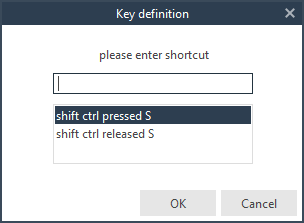
\includegraphics[width=140px]{../img/Alter-Editor.PNG}
	\caption{Bestehender Editor}
	\label{fig:existEditor}
\end{wrapfigure}

\subsection{Ist-Analyse}

Aktuell existiert bereits ein Editor zur Eingabe von Shortcuts (siehe \autoref{fig:existEditor}). Dieser ist allerdings sehr einfach aufgebaut und beschränkt sich auf die Eingabe eines Shortcuts per Tastatur. Außerdem ist es nicht möglich Warnungen anzuzeigen oder zwischen bestehenden Shortcuts zu navigieren.

\subsection{Soll-Analyse}



\vfill

\begin{figure}[H] 
	\subfigure{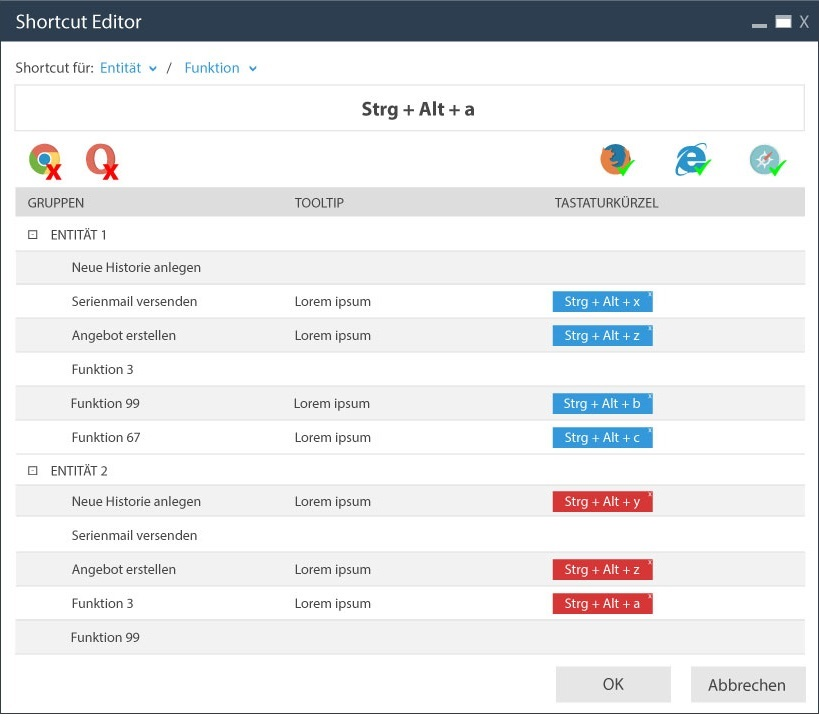
\includegraphics[width=0.5\textwidth]{../img/ux/2-ShortCutEditor-Eingabe.jpg}} 
	\subfigure{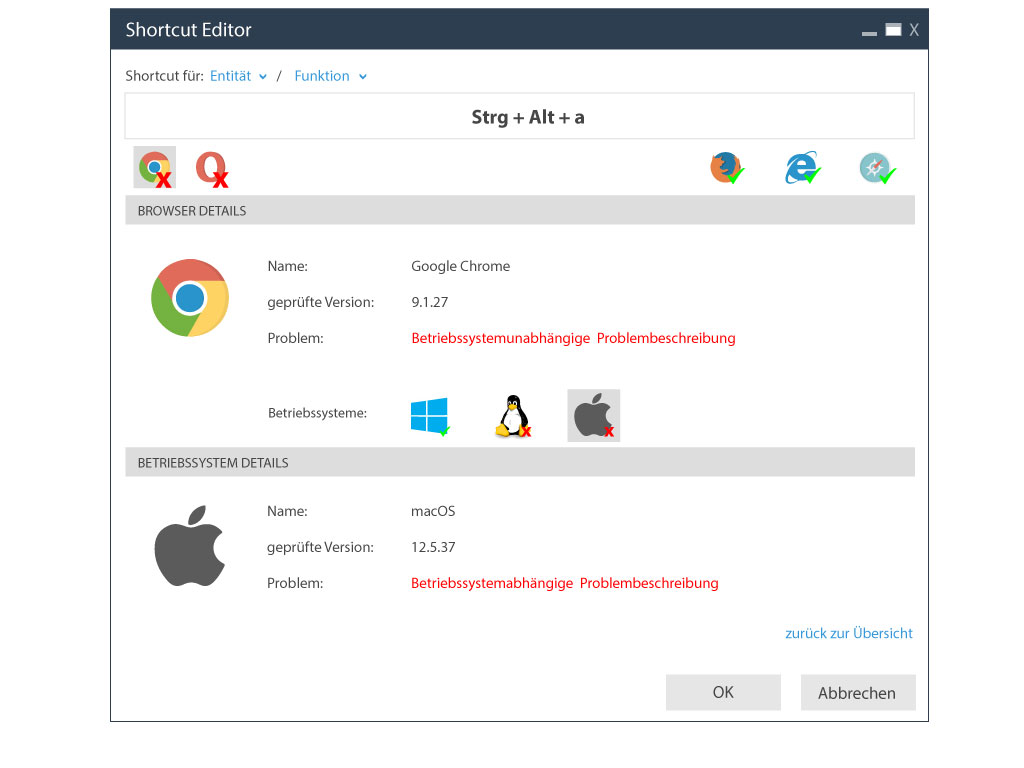
\includegraphics[width=0.5\textwidth]{../img/ux/4-ShortCut-Info.jpg}}
	\caption{UX-Entwürfe} 
\end{figure}

\newpage